\section{Auswertung}
\subsection{Vorbereitung}
Als Vorbereitung wird zunächst die Schallgeschwindigkeiten von einigen Materialien bestimmt. Diese sind in
der Tabelle (\ref{tab:1}) dargestellt.
\begin{table}[H]
  \centering
  \caption{Literaturwerte für Schallgeschwindigkeiten \cite{2} \cite{3}.}
  \label{tab:1}
  \begin{tabular}{c c}
    \toprule
     & $c \, / \, \si[per-mode=fraction]{\meter\per\second}$\\
     \midrule
     Luft \SI{0}{\celsius}          & 331  \\
     dest. Wasser \SI{20}{\celsius} & 1485 \\
     Acryl                          & 2730 \\
     \bottomrule
  \end{tabular}
\end{table}

\subsection{Untersuchung eines Acrylblocks mit dem A-Scan}
Zunächst werden die Abmessungen eines Acrylblocks mithilfe einer Schieblehre gemessen und in
der Tabelle (\ref{tab:2}) dargestellt.

\begin{table}[H]
  \centering
  \caption{Abmessung des Acrylblocks.}
  \label{tab:2}
  \begin{tabular}{c c c}
    \toprule
     $\text{Länge} \,/\, \si[per-mode=fraction]{\milli\meter}$ &$\text{Höhe} \, /\, \si[per-mode=fraction]{\milli\meter}$ &$\text{Breite} \, /\, \si[per-mode=fraction]{\milli\meter}$\\
     \midrule
     150 & 80.01 & 60 \\
     \bottomrule
  \end{tabular}
\end{table}

Anschließend werden die Tiefen der Fehlstellen mit dem A-Scan bestimmt. Die zugehörige Schallgeschwindigkeit
von Acryl wird von der Tabelle (\ref{tab:1}) entnommen und mit der Formel (\ref{eq:1}) wird der Ort der Fehlstellen bestimmt.
Um eine genau Lokalisation der Fehlstelle zu bekommen wird der Block zusätzlich von der andere Seite durchschallt.
Die Messaufnahmen sind in der Tabelle (\ref{tab:3}) dargestellt.

\begin{table}[H]
  \centering
  \caption{Messergebnisse vom A-Scan.}
  \label{tab:3}
  \begin{tabular}{c c c c}
    \toprule
    \multicolumn{2}{c}{Oben} & \multicolumn{2}{c}{Unten} \\
    \cmidrule(lr){1-2}\cmidrule(lr){3-4}
    $\text{Lochnummer}$ & $\text{Tiefe} \,/\, \si[per-mode=fraction]{\milli\meter}$ & $\text{Lochnummer}$ & $\text{Tiefe} \,/\, \si[per-mode=fraction]{\milli\meter}$\\
    \midrule
    11  & 56 & 11 & 15\\
    10  & 7  & 10 & 71\\
    9   & 16 & 9 & 63\\
    8   & 23 & 8 & 55\\
    7   & 31 & 7 & 47\\
    6   & 39 & 6 & 39\\
    5   & 47 & 5 & 30\\
    4   & 54 & 4 & 22\\
    3   & 62 & 3 & 13\\
    2   & 18 & 2 & 64\\
    1   & 22 & 1 & 60\\
  \bottomrule
  \end{tabular}
\end{table}

Der Durchmesser der jeweiligen Fehlstellen wird mit
\begin{itemize}
  \item $\diameter = |\text{Höhe} - (\text{Messwert}_{\text{Oben}} + \text{Messwert}_{\text{Unten}} )|$
\end{itemize}
berechnet und in der Tabelle (\ref{tab:4}) mit den tatsächlichen Abmessungen gegenübergestellt.
Für die Abweichung wird die folgende Formel verwendet.
\begin{itemize}
  \item $\text{Abweichung} = |\frac{\diameter_{Schieb} - \diameter_{Mess}}{\diameter_{Schieb}}| \cdot 100 \, \%$
\end{itemize}

\begin{table}[H]
  \centering
  \caption{Darstellung der Fehlerabweichung.}
  \label{tab:4}
  \begin{tabular}{c c c  c}
    \toprule
     $\text{Lochnummer}$ &
     $\diameter_{\text{Schieb}} \,/\, \si[per-mode=fraction]{\milli\meter}$ &
     $\diameter_{\text{Messung}} \,/\, \si[per-mode=fraction]{\milli\meter}$ &
     $\text{Abweichung} \,/\, \%$ \\
     \midrule
     1 & 1,25 & 2 &  60 \\
     2 & 1,25 & 2 &  60 \\
     3 & 5,30 & 5 &  6 \\
     4 & 4,30 & 4 &  7 \\
     5 & 3,40 & 3 &  12 \\
     6 & 2,45 & 2 &  18 \\
     7 & 2,45 & 2 &  18 \\
     8 & 2,45 & 2 &  18 \\
     9 & 2,45 & 1 &  51 \\
     10 & 2,45 & 2 & 18\\
     11 & 9,35  & 9 & 4 \\
     \bottomrule
  \end{tabular}
\end{table}

\subsection{Untersuchung des Auflösungsvermögens}
In dieser Versuchsreihe soll die Auflösung mit unterschiedlichen Sonden, an den Fehlstellen mit
der Lochnummer 1 und 2, untersucht werden.
Die Aufnahmen werden mit jeweils einer 1 GHz, 2 GHz und 4 GHz Sonde durchgeführt. Die Aufnahmen werden
in den Abbildungen (\ref{abb:2}), (\ref{abb:3}) und (\ref{abb:4}) dargestellt.

\begin{figure}[H]
  \centering
  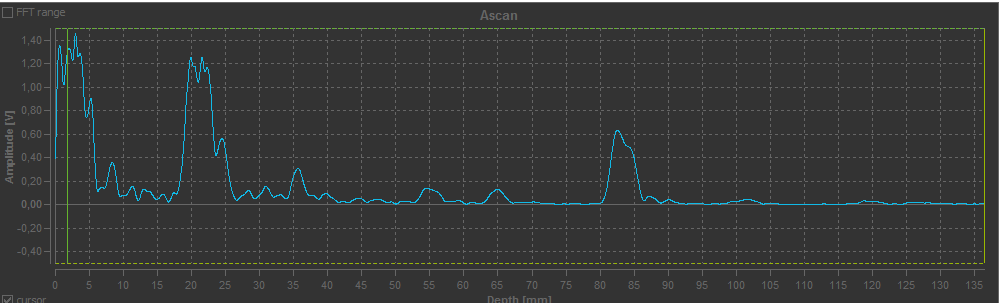
\includegraphics[width=\textwidth]{content/1MHz.png}
  \caption{Aufnahme mit der 1 GHz Sonde.}
  \label{abb:2}
\end{figure}

\begin{figure}[H]
  \centering
  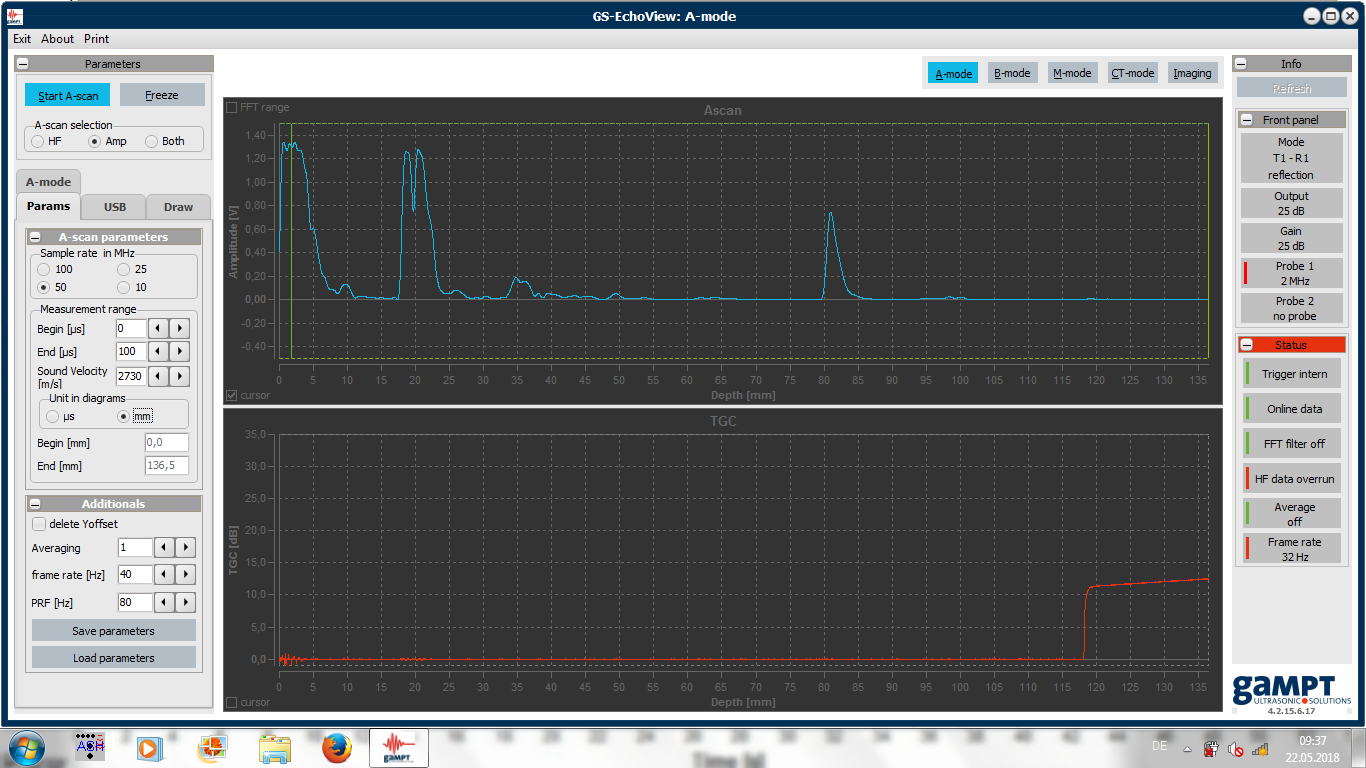
\includegraphics[width=\textwidth]{content/2MHz.png}
  \caption{Aufnahme mit der 2 GHz Sonde.}
  \label{abb:3}
\end{figure}

\begin{figure}[H]
  \centering
  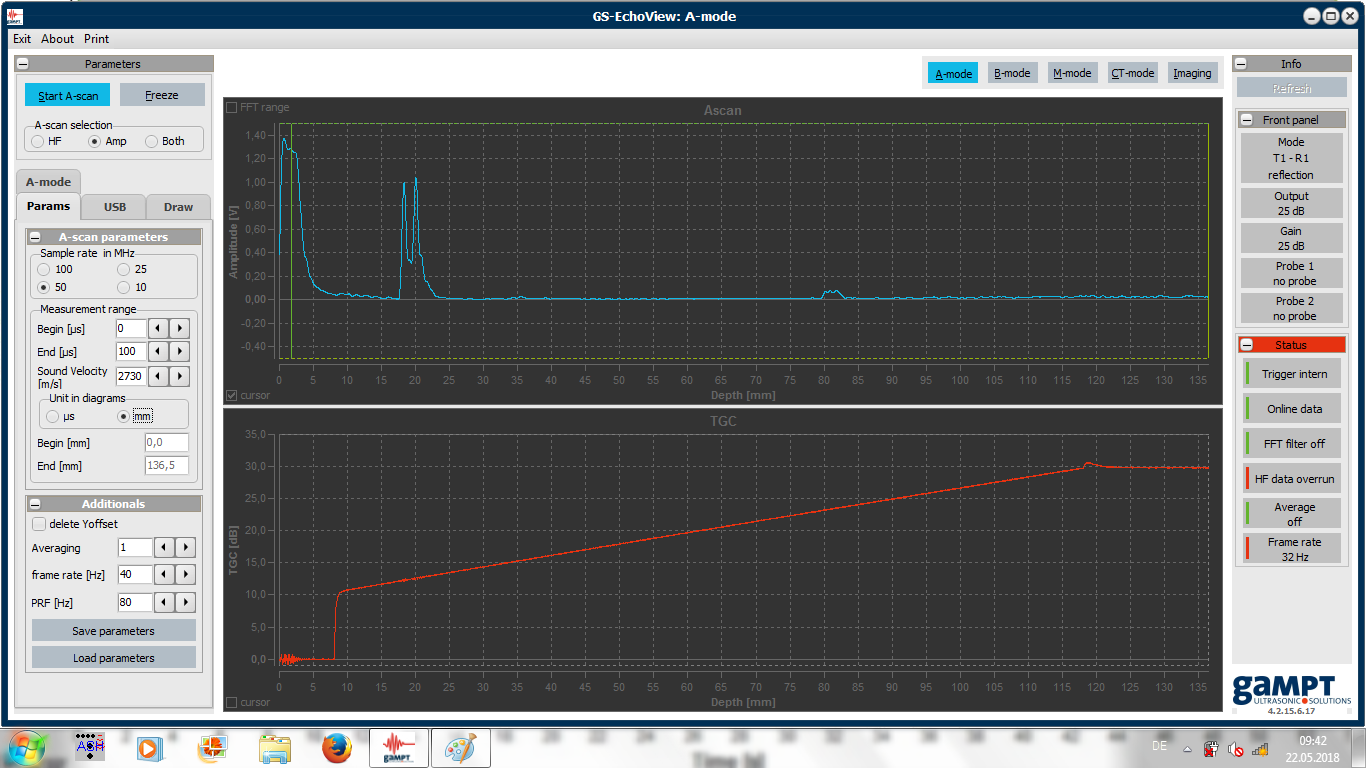
\includegraphics[width=\textwidth]{content/4MHz.png}
  \caption{Aufnahme mit der 4 GHz Sonde.}
  \label{abb:4}
\end{figure}

\subsection{Untersuchung eines Acrylblocks mit dem B-Scan}
Nun werden die Fehlstellen mit einem B-Scan untersucht.
Dabei wird der Block von beiden Seite durchschallt um dann
den Durchmesser der Fehlstellen ermitteln zu können.
In den Abbildungen (\ref{abb:5}) und (\ref{abb:6}) sind die Aufnahmen
vom B-Scan dargestellt.

\begin{figure}[H]
  \centering
  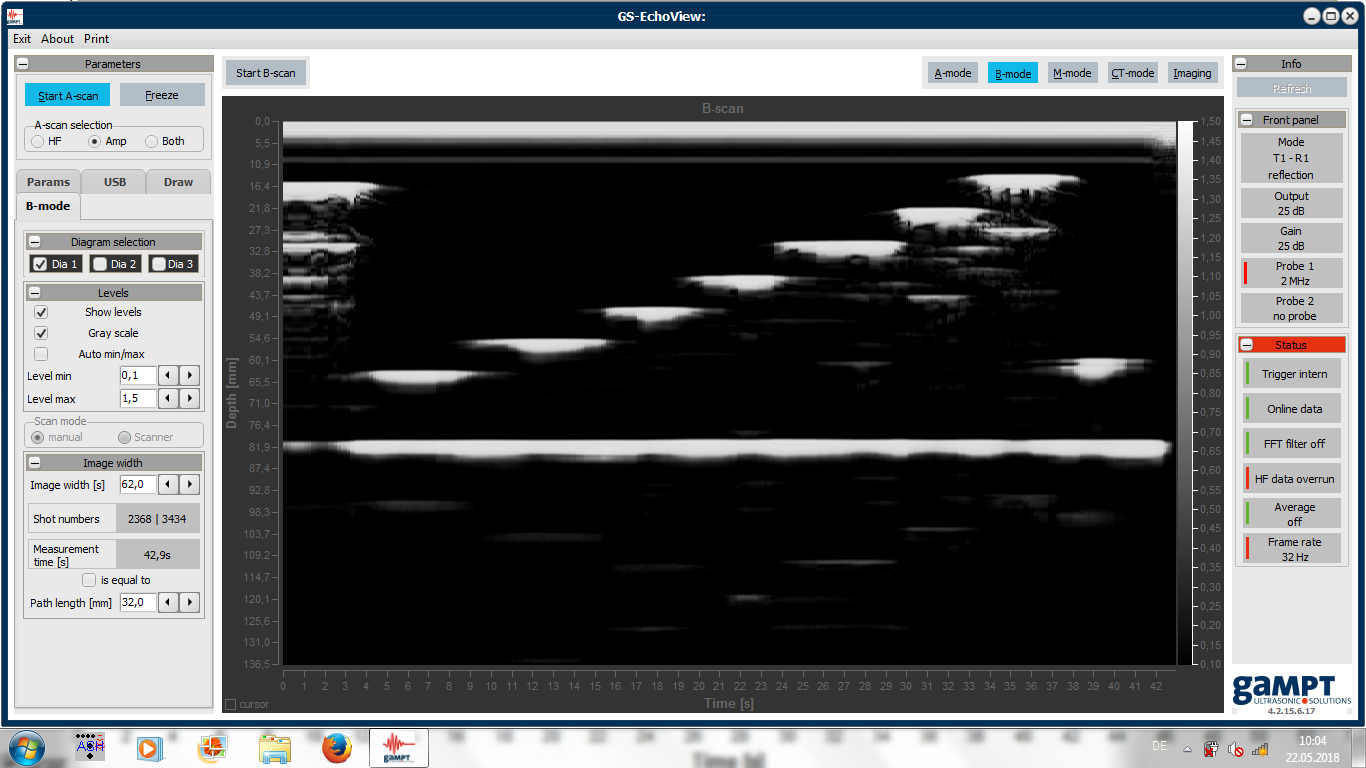
\includegraphics[width=\textwidth]{content/B-Scan2.png}
  \caption{Darstellung vom B-Scan (Oben).}
  \label{abb:5}
\end{figure}
\begin{figure}[H]
  \centering
  \includegraphics[width=\textwidth]{content/B-Scan1.png}
  \caption{Darstellung vom B-Scan (Unten).}
  \label{abb:6}
\end{figure}
Aus den Aufnahmen wird nun die Lage der Fehlstellen entnommen und es wird
anschließend der Durchmesser mit der oben erwähnten Formel berechnet. Die Daten werden
in der Tabelle (\ref{tab:5}) dargestellt.
\begin{table}[H]
  \centering
  \caption{Durchmesser der jeweiligen Fehlstellen.}
  \label{tab:5}
  \begin{tabular}{c c c c c}
    \toprule
     $\text{Lochnummer}$ &
     $\text{Lage}_{\text{Oben}} \,/\, \si[per-mode=fraction]{\milli\meter}$ &
     $\text{Lage}_{\text{Unten}} \,/\, \si[per-mode=fraction]{\milli\meter}$ &
     $\diameter_{\text{Messung}} \,/\, \si[per-mode=fraction]{\milli\meter}$ \\
     \midrule
     1 & 17,9 & 59,6 & 2,5\\
     2 & 18,1 & 59,8 & 2,1\\
     3 & 61,1 & 13,6 & 5,3\\
     4 & 53,8 & 22,1 & 4,1\\
     5 & 46,3 & 29,9 & 3,8\\
     6 & 39,0 & 39,0 & 2,0\\
     7 & 30,9 & 47,0 & 2,1\\
     8 & 22,9 & 54,8 & 2,3\\
     9 & 15,1 & 62,6 & 2,3\\
     10 & 7,3 & 71,2 & 1,5\\
     11 & 55,3& 15,4 & 9,3\\
     \bottomrule
  \end{tabular}
\end{table}
Mit der oben erwähnten Fehlerformel werden die Abweichungen von dem mit der Schieblehre
ermittelten Durchmessern zu den Messwerten
bestimmt und in der Tabelle (\ref{tab:6}) dargestellt.
\begin{table}[H]
  \centering
  \caption{Darstellung der Fehlerabweichung.}
  \label{tab:6}
  \begin{tabular}{c c c  c}
    \toprule
     $\text{Lochnummer}$ &
     $\diameter_{\text{Schieb}} \,/\, \si[per-mode=fraction]{\milli\meter}$ &
     $\diameter_{\text{Messung}} \,/\, \si[per-mode=fraction]{\milli\meter}$ &
     $\text{Abweichung} \,/\, \%$ \\
     \midrule
     1 &  1,25  & 2,50 & 100    \\
     2 &  1,25  & 2,10 & 86,6   \\
     3 &  5,30  & 5,30 & 0      \\
     4 &  4,30  & 4,10 & 4,7    \\
     5 &  3,40  & 3,80 & 11,8   \\
     6 &  2,45  & 2,00 & 18,4   \\
     7 &  2,45  & 2,10 & 14,3   \\
     8 &  2,45  & 2,30 & 6,1    \\
     9 &  2,45  & 2,30 & 6,1    \\
     10 & 2,45 & 1,50 &  39,6   \\
     11 & 9,35 & 9,30 &  0,5    \\
     \bottomrule
  \end{tabular}
\end{table}

\subsection{Untersuchung eines Herzmodells mit dem TM-Scan}
Zunächst wird die Laufzeit des Echos mit einem A-Scan durchgeführt.
Sie beträgt $\Delta t = 54,1 \, \mu s$.
Nun wird mithilfe eines Time-Motion Scans die Herzfrequenz aufgenommen und
in der Abbildung (\ref{abb:7}) dargestellt.
\begin{figure}[H]
  \centering
  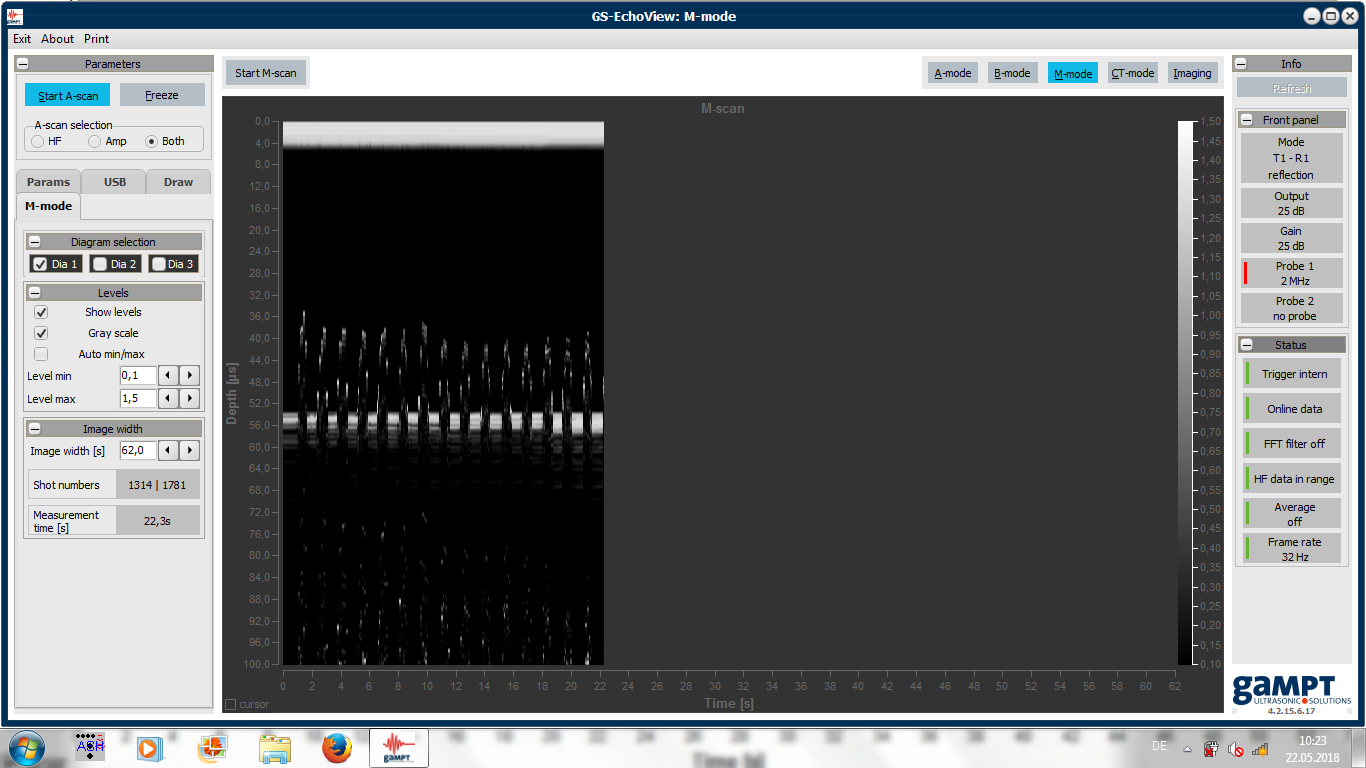
\includegraphics[width=\textwidth]{content/HZV.png}
  \caption{Darstellung der Herzfrequenz mit dem TM-Scan.}
  \label{abb:7}
\end{figure}
Es muss die Annahme gemacht werden, dass der enddiastolische Wert null ist.
Für das Zeitintervall geht aus der Abbildung (\ref{abb:7}) hervor:

\begin{itemize}
  \item $t_{\text{INT}} = 22,1 \, \si{\second}$
\end{itemize}

In diesem Zeitintervall gab es $15$ Schläge.
Somit ergibt sich für die Herzfrequenz:

\begin{itemize}
  \item $v_{\text{Herz}} = \frac{15}{22,1} \si{\per\second} = 0,68 \si{\per\second}$
\end{itemize}

In der folgenden Tabelle (\ref{tab:7}) wird mithilfe der Formel (\ref{eq:2}) das Herzzeitvolumen
bestimmt. Für den endsystolischen Wert werden die Amplituden aus der Abbildung (\ref{abb:7}) analysiert und
ausgewertet. Dabei ist die Nulllinie die Laufzeit $\Delta t = 54,1 \, \mu s$ vom Echo.

\begin{table}[H]
  \centering
  \caption{Darstellung des Herzzeitvolumens mit $\text{EDV} =0$.}
  \label{tab:7}
  \begin{tabular}{c c}
    \toprule
     $\text{EDS}\,/\,\si{\milli\litre}$ &
     $\text{HZV} \,/\, \si[per-mode=fraction]{\milli\litre\per\second}$ \\
     \midrule
      19,1 & 12,99 \\
      16,1 & 10,95\\
      16,1 & 10,95\\
      15,1 & 10,27\\
      16,1 & 10,95\\
      16,1 & 10,95\\
      17,1 & 11,63\\
      14,1 & 9,59\\
      14,1 & 9,59\\
      13,1 & 8,91\\
      14,1 & 9,59\\
      13,1 & 8,91\\
      14,1 & 9,59\\
      14,1 & 9,59\\
      15,1 & 10,27\\
     \bottomrule
  \end{tabular}
\end{table}
Diese Werte werden nun gemittelt.
Für den Mittelwert und die Standardabweichung werden die Formeln \ref{fel:1} und \ref{fel:2} verwendet.
\begin{equation}
    \bar{x} = \frac{1}{N} \sum_{i=1}^{N} x_i
    \label{fel:1}
\end{equation}
\begin{equation}
  \Delta \bar{x} = \frac{1}{\sqrt{N}\sqrt{N-1}} \sqrt{\sum_{i}(x_i-\bar{x})^2}
  \label{fel:2}
\end{equation}

\begin{itemize}
  \item $\text{EDV} = 15,17 \pm 0,42\, \si{\milli\litre}$
  \item $\text{HZV} = 10,32 \pm 0,29\, \si{\milli\litre\per\second}$
\end{itemize}
